\chapter{The Hall effects}

\label{chapter2}

\section{Introduction - Ordinary Hall effect} \label{sec:ohe}

These effects originally deal with the application of an external magnetic field on a current carrying material and subsequently observing the effect either on the conductor or the electric current itself.

In 1879, Edwin Hall was exploring this interaction and tried to determine the effect of the magnetic field on a current carrying wire, with a suspicion that it either affected the whole length of the wire or only the moving electrons.

He later devised a rather simple experiment based on the argument that ``if the current of electricity in a fixed conductor is itself attracted by a magnet, the current should be drawn to one side of the wire, and therefore the resistance experienced should be increased." \cite{S.1880}

Hall couldn't detect this extra resistance (which we now know as magnetoresistance) but concluded that a transverse force in the opposite direction must exist and which appears as a transverse voltage across the width of the conducting material.
This is the Hall effect and the transverse voltage is the Hall voltage.

The experiment by Hall is shown in the figure below.

\begin{figure}[h!]
    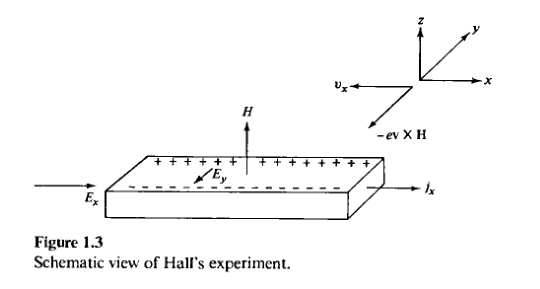
\includegraphics[width=0.7\columnwidth]{hall-effect-ashcroft.png}
    \caption{Schematic diagram of the Hall effect\\ \textit{Image credit: Ashcroft \& Mermin, Solid State Physics}  }
    \label{hall-figure}
\end{figure}

\begin{figure}[h!]
    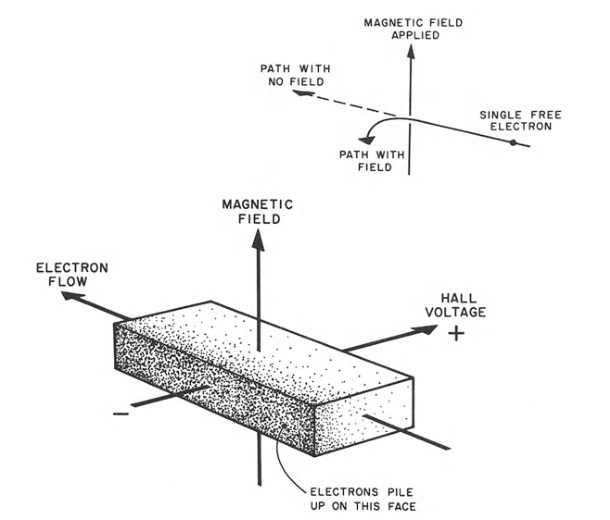
\includegraphics[width=\columnwidth]{hall-effect-hurd.png}
    \caption{A more "self-explanatory" diagram of the Hall effect\\ \textit{Image credit: C.M Hurd, The Hall effect in metals and alloys}}
\end{figure}

\subsection{Mechanism of OHE}

In the \cref{hall-figure} , an electric current is passed along the $ x $ direction with corresponding current density is $ j_x $.
The cause of this current is an external electric field along the same direction, $ E_x $.

An external magnetic field $ H $ along the $ z $ direction is applied and the Hall effect is observed.

From the Lorentz force equation

\begin{equation} \label{lorentz}
    \vec{F} = q (\vec{E} + \vec{v} \times \vec{H})
\end{equation}

The second term of the \cref{lorentz} is responsible for deflecting the trajectory of the electrons in the negative $ y $-direction and accumulating along the sides of the material.
As this accumulation takes place, an electric field builds up along the $ y $-direction which opposes the further deflection of electrons towards the sides.
This process continues until an equilibrium is reached, at which this transverse field (or \textbf{Hall field}) $ E_y $ perfectly balances the Lorentz force and the current flows only along the longitudinal direction \cite{ashcroft1976solid}.

\subsection{Hall coefficient}

This transverse Hall field $ E_y $ can be thought of to be proportional to the external magnetic field $ H $ and longitudinal current density $ j_x $.
Here, we define the Hall coefficient as

\begin{equation} \label{hall-coeff}
    R_H = \frac{E_y}{j_x H}
\end{equation}

A rather interesting point to note is that by our construction, $ j_x $ and $ H $ are along positive $ x $ and $ z $ directions respectively.
$ E_y $ however, is along negative $ y $ direction, meaning that the resultant sign of the Hall coefficient $ R_H $ is negative.

Now, imagine if the charge carriers were positive, this would result in their velocity along $ x $-direction to get reversed ($ j_x $ would still be along positive $ x $-direction).
The Lorentz force would remain unchanged (as can be seen from \cref{lorentz}).
Consequentially, the direction of Hall field would be in the opposite direction compared to its direction in the case of negatively charged carriers.
This would mean that measuring the Hall coefficient of a material, would help one determine the sign of the charge carriers \cite{ashcroft1976solid}.

\subsubsection{Calculating the Hall coefficient}

Let us consider current densities $ j_x $ and $ j_y $ in the presence of an electric field with components $ E_x $ and $ E_y $, and in the presence of an external magnetic field $ H $ along the $ z $-axis.

The average force per electron is given by the Lorentz force equation, i.e. $ \vec{F} = -e (\vec{E} + \vec{v} \times \vec{H}) $, and hence the average momentum per electron becomes

\begin{equation}
    \frac{d \vec{p}}{dt} = -e \left( \vec{E} + \frac{\vec{p}}{m} \times H \right) - \frac{\vec{p}}{\tau}
\end{equation}

During equilibrium, the current becomes time-independent, and hence $ p_x $ and $ p_y $ satisfy the equations

\begin{equation}
    \begin{split}
        0 &= -e E_x - \omega_c p_y - \frac{p_x}{\tau}\\
        0 &= -e E_y + \omega_c p_x - \frac{p_y}{\tau}
    \end{split}
\end{equation}

where

\begin{equation}
    \omega_c = \frac{e H}{m}
\end{equation}

Solving the above equations, we get

\begin{equation}
    E_y = - \left( \frac{\omega_c \tau}{\sigma_0}  \right) j_x = - \left( \frac{H}{ne} \right) j_x
\end{equation}

This yields the Hall coefficient (\cref{hall-coeff}) to be

\begin{equation}
    \boxed{R_H = - \frac{1}{ne}}
\end{equation}

where $ n $ is the number density of the charge carriers.

This is a rather astonishing result, suggesting that the Hall coefficient of a material, depends solely on the density of the carriers \cite{ashcroft1976solid}.

We then define Hall resistivity $ \rho_H $ as the Hall field $ E_y $ per unit longitudinal current density $ j_x $, which is given by

\begin{equation} \label{hall-resistivity}
    \boxed{\rho_H = \frac{E_H}{j_x} = R_H H}
\end{equation}

where the symbols have their usual meanings.

We shall stop our investigation of the Ordinary Hall effect in lieu of the main topic of the report.

\section{Anomalous Hall effect (AHE)}

The previous section dealt with OHE where the nature of the current carrying material is immaterial.
Now, we deal with specific characteristics of such material, namely, magnetic metals.

It is observed that when observing Hall effect in such magnetic materials, in addition to OHE, certain unusual phenomena are observed.

In low-field conditions as seen from \cref{hall-resistivity}, the observed Hall resistivity $ \rho_H $ varies linearly with external magnetic field $ H $ with the slope given by the Hall coefficient $ R_H $.
For illustration purposes, the example of Hall resistivity $ \rho_H $ has been used.
The trend is the same for Hall field $ E_H $ as can be observed from \cref{hall-resistivity}.

What about magnetic metals?
In such materials, a linear but rapid rise in the Hall field is seen with increasing external magnetic field $ \vec{H} $.
This is followed by a secondary linear rise (with a lower gradient compared to the first), which later saturates at large fields and becomes almost independent of the external field.
This is depicted in \cref{fig:hall-rho-linear}

\begin{figure}[h!]
    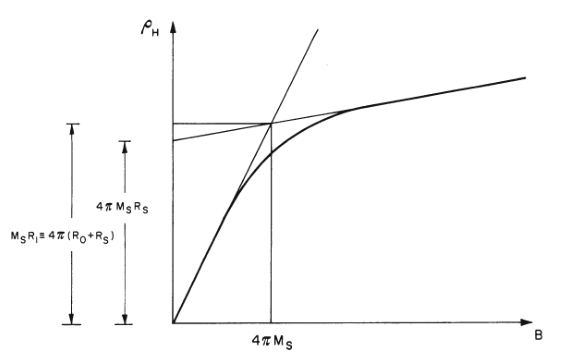
\includegraphics[width=\columnwidth]{hall-rho-hurd.png}
    \caption{Schematic behaviour of the Hall resistivity $ \rho_H $ as a function of magnetic induction $ \vec{B} $ in a metal showing appreciable magnetization.\\ \vspace{0.2cm} \textit{Image credit: C.M Hurd, The Hall effect in metals and alloys.} }
    \label{fig:hall-rho-linear}
\end{figure}

In this case, the Hall effect is not simply from the application of Lorentz force on the charge carriers but rather seen as an \textit{anomaly} and is therefore known as the \textbf{anomalous Hall effect.}


\subsection{Mechanism of AHE}

It has been shown empirically that this anomalous behaviour can be explained by a superposition of OHE and a strongly temperature dependent term.
The curve shown in \cref{fig:hall-rho-linear}
can be empirically fitted by the following equation (in CGS units):

\begin{equation} \label{ahe}
    \rho_H = R_0 B + \mu_0 R_s M
\end{equation}

where $ B $ is the applied magnetic field, $ R_0 $ is the ordinary Hall coefficient, $ M $ is the magnetization of the material, $ R_s $ is the anomalous Hall coefficient and \( \mu_0 \) is the permeability of free space.

The first term in \cref{ahe} accounts for OHE and is characterized by the more familiar \cref{hall-resistivity}, whereas the second term is a characteristic of magnetic materials.
This magnetization $ \vec{M} $ can be present even without the presence of an external magnetic field $ \vec{B} $, especially in ferromagnetic materials.

Especially in the case of ferromagnets, $ R_s $ is experimentally found to be strongly temperature dependent.














\section{Spin Hall effect (SHE)} \label{sec:she}

In this type of Hall effect, we generally deal with non-magnetic (or weakly magnetic) materials.
For example, a paramagnetic material or a ferromagnetic material beyond its Curie temperature.
Strictly speaking, an external magnetic field is not \textit{mandatory} to observed SHE.

When a charge current is supplied in a specific direction along a conducting material, an addition parameter of the charge carriers, namely, the spin of the electrons is responsible for a unique phenomena to take place.
If these electrons have the directions of their spins along specific directions (in our interest, spins perpendicular to the plane of the conducting material), then such electrons are \textit{spin-polarized} and via scattering mechanisms\footnotemark, these electrons get preferentially scattered, giving rise to a spin current \cite{dyakonov1971current,hirsch1999spin}.

In layman terms, SHE reduces to the following: \textit{Spin accumulation at the lateral boundaries of the material, with the directions of spins being opposite at the opposing sides.}

This phenomena is very similar and analogous to OHE, the only difference being that instead of opposite charge accumulation on lateral sides, electrons with opposite spins get accumulated.

We shall discuss the plausible mechanisms responsible for the spin Hall effect in greater detail in the forthcoming chapters.

\subsection{Spin Current}

A pure spin current can be defined as the flow of electrons of spin $ \uparrow $ moving in one direction and electrons of the opposite spin i.e. $ \downarrow $ electrons moving along the opposite direction.
This results in no net charge current (since rate of movement of electrons in opposing directions is the same) and a net flow of angular momentum \cite{krishnan2016fundamentals}.

\subsubsection{Mathematical analysis}

From the continuity equation,

\begin{equation} \label{continuity}
    \nabla \vec{J} + \frac{\partial \rho}{\partial t} = 0
\end{equation}

where $ \vec{J} $ is the current density and $ \rho $ is the charge density.

This \cref{continuity} implies charge conservation law and helps us define the charge current \cite{jackson1999classical}.

Analogously, we can define the spin current density $ \vec{J}_s $ with reference to conservation of spin angular momentum. Considering that spin angular momentum is conserved, we can then define the corresponding continuity equation as

\begin{equation} \label{spin-current-density}
    \nabla \vec{J}_s + \frac{\partial \vec{M}}{\partial t} = 0
\end{equation}

where $ \vec{M} $ is the magnetization (magnetic moment per unit volume) of the sample. The \cref{spin-current-density} defines the spin current density $ \vec{j}_s $ \cite{Uchida_2016}.

\begin{figure}[h!]
    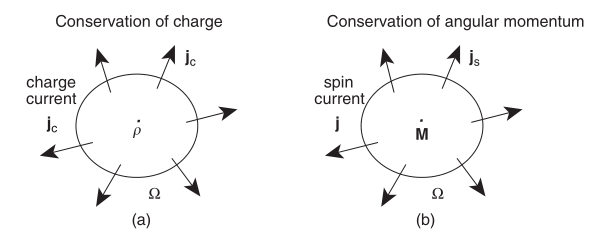
\includegraphics[width=\columnwidth]{spin-current.png}
    \caption{The total sum of rate of all charge variations across a surface is equal to the total current entering the surface.\\ \vspace{0.2cm} \textit{Image credit: "Spin Current", Ken-ichi Uchida and Eiji Saitoh}}
\end{figure}


In real solids for most of the cases, the conservation of spin angular momentum is a good approximation. However, in general, the conservation does not hold true due to spin relaxation (due to collisions with impurities in the solid, the spins of the electrons does not remain polazized) \cite{Uchida_2016}. This gives rise to a modified version of \cref{spin-current-density} as:

\begin{equation}
    \nabla \vec{J}_s + \frac{\partial \vec{M}}{\partial t} = -\vec{T}
\end{equation}

where $ \vec{T} $ is an indicator of the non-conservation of spin angular momentum (due to spin relaxation and spin generation) \cite{Uchida_2016}.

\section{Inverse Spin Hall effect (ISHE)}

Contrary to SHE, the inverse Hall effect is essentially the same but SHE in reverse. When a pure spin current is injected into a material (with no charge current), the same scattering mechanisms\footnotemark[\value{footnote}] in case of SHE, allow the spin-polarized electrons to preferentially scatter into opposite directions.

The spin $\uparrow$ electrons scatter along one direction and the spin $\downarrow$ electrons scatter along another direction. The surprising aspect about this, is that \textbf{both the directions are the same!}
This leads to a pure charge current.

The \cref{she-vs-ishe} is a schematic representation of the phenomena:

\begin{figure}[h!]
    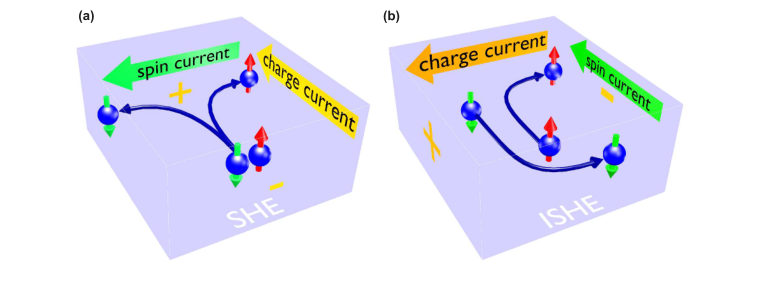
\includegraphics[width=\columnwidth]{ishe.png}
    \caption{Comparison between SHE and ISHE.\\ \vspace{0.2cm}\textit{Image credit: M.B Jungfleisch, PhD Thesis}}
    \label{she-vs-ishe}
\end{figure}

\footnotetext{We shall discuss the plausible mechanisms responsible for the spin Hall effect in greater detail in the forthcoming chapters.}
